\documentclass[../workflow.tex]{subfiles}
\graphicspath{{\subfix{../img/}}}

\begin{document}
    \section{General Notes}

    \etocignoretoctocdepth % of course, if we want to see something in local TOC...
    \etocsettocstyle{\subsection*{\contentsname}}{}
    \localtableofcontents
    
    \subsection{Notes from Books/Papers}

    \begin{note}[]
        [In this equation...] the time evolution depends only on the present state of the
        system, and is defined entirely by knowledge of the set of transition probabilities.
        Such systems are called \it{Markovian systems}.
    \end{note}


    \subsection{Handwritten Notes}
    
    \begin{figure}[H]
        \centering
        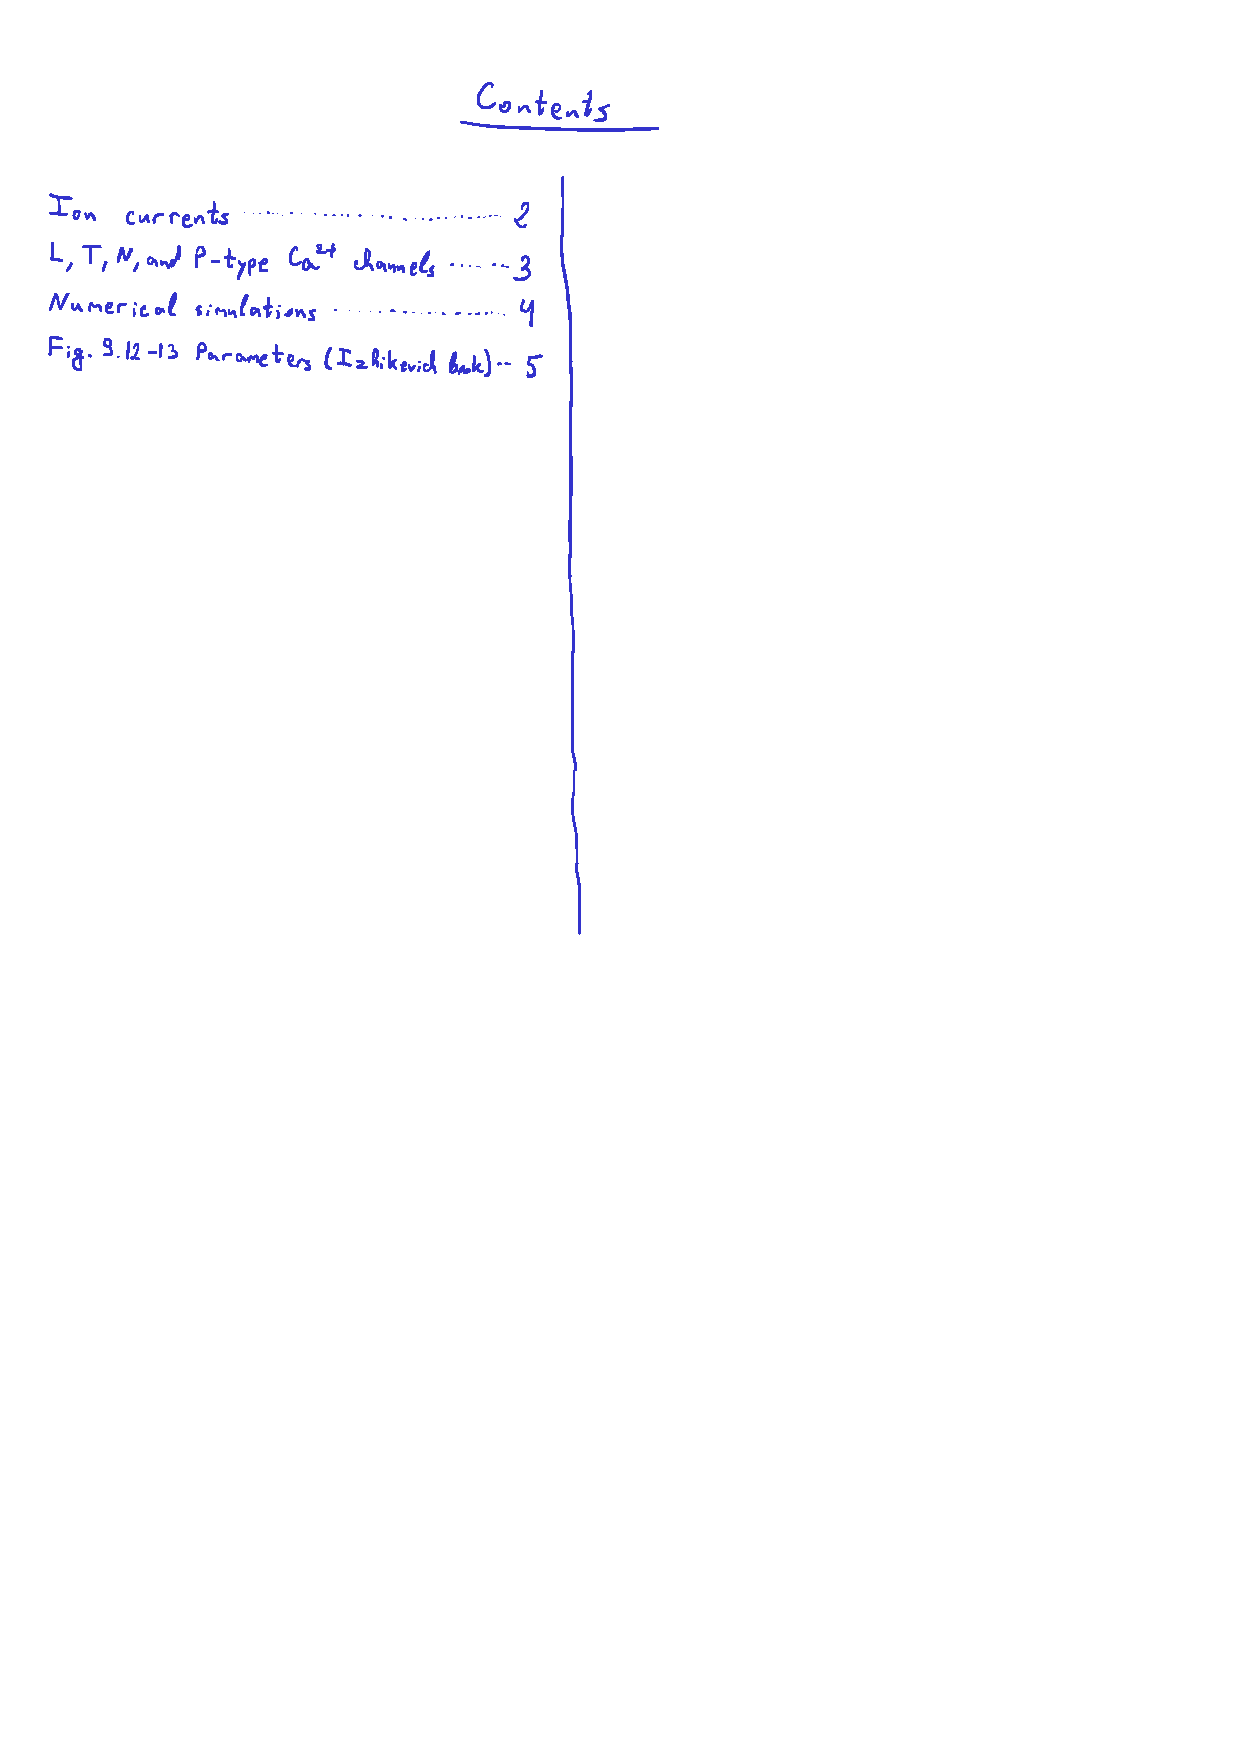
\includegraphics[height=0.95\textheight, page=1]{Handwritten Notes/General Notes.pdf}
    \end{figure}
    
    
    % Insert the PDF and apply custom page numbering for the footer
    \includepdf[pages=2-,height=\textheight,pagecommand={
      \thispagestyle{mypdfstyle}  % Apply custom footer with page number
    }]{Handwritten Notes/General Notes.pdf}

\end{document}
